\documentclass{article}

\usepackage{graphicx} % more modern
\usepackage{subfigure} 
\usepackage{amssymb}
\usepackage{amsmath}
\usepackage{amsthm}


% For citations
\usepackage{natbib}

% For algorithms
\usepackage{comment}
\usepackage{framed}
\usepackage{algorithm}
\usepackage{algorithmic}
\usepackage{amsmath}
%\usepackage{algorithmicx}
%\usepackage{algpseudocode}

\usepackage{hyperref}

\allowdisplaybreaks

\newcommand{\theHalgorithm}{\arabic{algorithm}}

\newtheorem{theorem}{Theorem}[section]
\newtheorem{lemma}[theorem]{Lemma}
\newtheorem{conjecture}[theorem]{Conjecture}
\newtheorem{proposition}[theorem]{Proposition}
\newtheorem{definition}[theorem]{Definition}
\newtheorem{corollary}[theorem]{Corollary}

\usepackage[accepted]{icml2014}  % XXX : just set temporarly to print out authors corretly.
%\usepackage{icml2014}  

\renewcommand{\algorithmicrequire}{\textbf{Input:}}
\renewcommand{\algorithmicensure}{\textbf{Output:}}

\begin{document} 

\icmltitle{Exploiting Redundancies in Convolutional Networks}

\icmlauthor{Emily Denton}{denton@cs.nyu.edu}
\icmlauthor{Wojciech Zaremba}{zaremba@cs.nyu.edu}
\icmlauthor{Joan Bruna}{bruna@cs.nyu.edu}
\icmlauthor{Rob Fergus}{fergus@cs.nyu.edu}

\icmlkeywords{machine learning, deep learning, speeding up forward pass, redundancies in neural networks}

\begin{abstract}

\end{abstract}

\section{Introduction}

Training large neural networks (NN) takes weeks, or even months. This can hinder 
research, and there have been extensive effort devoted to speed up training procedure.
However, resource-wise from perspective of companies executing neural networks on internet-scale
data (e.g. annotating images), this is not the main cost. Major cost is in the
final stage, where network is evaluated on the target data, which is present in quantities of billions.
We focus here on speeding up evaluation of \emph{trained} NN, which directly
maps to the cost of executing NN on internet-scale data. Our techniques speed up execution by 
factor of $2-4$ while keeping prediction accuracy within $1\%$ from the original model. 


% XXX: Maybe we will speak also about real time application.


We focus in this work on convolutional neural networks used for computer vision tasks. Most of
computation time during evaluation is spend on convolutional layers i.e. $\sim90\% - 95\%$, while it takes only
the small fraction of time $\sim 5\%-10\%$ to evaluate rest of layers (pooling, local contrast normalization,
fully connected). It is worth to note, that most of learnable parameters are kept in fully connected layers $\sim 90\% - 95\%$
, and convolutional layers constitutes of very small fraction of parameters $\sim 5\% - 10\%$.


We achieve forward pass speed up by constructing approximations to the convolutional layer kernel. Convolutional kernel
is a $4$-dimensional tensor, with two spacial dimensions, and two feature maps-to-feature maps dimensions. Kernel of trained
network has a lot of redundancies in parameters, which we exploit to speed up forward pass, while mildly training off
prediction accuracy (approximated kernels give prediction within $\sim 1\%$ of the original prediction).


\section{Related Work}
There have been extensive research devoted speeding up forward pass of neural network. 
There are few different pathways, how the speed up can be achieved. 


Vanhoucke et. al. \cite{vanhoucke2011improving} examined how to exploit properties of CPUs to speed up execution.
They present many solutions specific to Intel and AMD CPUs, however some of their propositions are general enough to be 
used for any type of processor.
They describe how to align memory, and use SIMD operations (vectorized operations on CPU) to get more efficient matrix multiplication. 
Moreover, they propose to use linearly quantize for weights, and input. Linear quantization
replaces 32-bit values of weights with 8-bits (range $[-128, 127]$). This approximation is similar
to our approach, which replaces kernel $W$ with few other operations, 
which give result approximately equal to convolution with $W$. Moreover, linear quantization
can be used in conjunction with methods presented in this paper.



Most expensive operation in neural networks for vision is convolution. Complexity of this operation
grows proportionally to the square size of local receptive field (in the direct, common implementation). 
However, Mathieu et. al. \cite{mathieu2013fast} shown that convolution can be efficiently
computed in Fourier domain, where it becomes element-wise multiplication (there is no cost
associated with size of receptive field). It is worth to note, that to operate in Fourier domain, 
one has to perform Fourier transform, and inverse Fourier transform to bring data back to original domain, which are
operations not without cost. They report speed up in forward pass up to $10x$ (depending on the kernel size, number of features etc.).
Moreover, this method can be used jointly with most of techniques presented in this paper.



Our low-rank approximations get inspired by work of Denil et. al \cite{denil2013predicting} on redundancies in neural 
networks. They shown that based on small fraction of weights (e.g. $\sim 5\%$), one can accurately 
predict rest of weights. This indicates that neural networks are heavily over-parametrized.
All the methods presented here focus on exploiting linear structure of this over-parametrization.


\section{Low Rank Approximations}
In this section, we give theoretical background on low rank approximations. First, we discuss simplest setting, which is
for matrices (two dimensional tensors). Further, we move to approximation of 4-dimensional tensors with 2 convolutional (spacial)
dimensions.


\subsection{Matrix Low Rank Approximation}
Let's consider input $X \in \mathbb{R}^{n \times m}$, and matrix of weights $W \in \mathbb{R}^{m \times k}$. Matrix multiplication
, which is the main operation for fully connected layers costs $O(nmk)$. However, potentially $W$ might have a low-rank (many 
eigenvalues close to zero), and operation $XW$ can be computed much faster. 


Every matrix can be expressed using singular value decomposition:
\begin{equation*}
	W = USV^T\text{, where }U \in \mathbb{R}^{m \times m}, S \in \mathbb{R}^{m \times k}, V \in \mathbb{R}^{k \times k}
\end{equation*}
$S$ is has eigenvalues on the diagonal, and apart from it has zeros. $W$ can be approximated by using $t$ most significant
eigenvalues from $S$. We can write approximation as
\begin{equation*}
	\hat{W} = \hat{U}\hat{S}\hat{V}^T\text{, where }\hat{U} \in \mathbb{R}^{m \times t}, \hat{S} \in \mathbb{R}^{t \times t}, \hat{V} \in \mathbb{R}^{t \times k}
\end{equation*}

Cost of multiplication $X$ with $\hat{W}$ is $O(nmt + nt^2 + ntk)$, which can be significantly smaller than $O(nmk)$ (for sufficiently small $t$). E.g.
for $n = 1000, m = 1000, k = 1000$ and $t = 100$, we have that exact computation takes $10^9$ operations, while the approximated one takes
$2 * 10^8 + 10^7$ operations. This would give $\times 5$ theoretical speed up. However, often major cost is in memory management, 
and theoretical speed up might be infeasible or very difficult to achieve. 


\subsection{Tensor Low Rank Approximations}

In typical object recognition architectures, the convolutional tensors resulting
from the training exhibit strong redundancy and regularity across all its 
dimensions. A particularly simple way to exploit such regularity is to 
linearly compress the tensors, which amounts to finding low-rank 
approximations.

Convolution kernels can be described as a $4$-dimensional tensors. Let $W \in \mathbb{R}^{C \times X \times Y \times F}$ 
be convolutional kernel. 
$C$ is input number of feature maps (or colors), $X, Y$ are special dimensions
over which we compute convolution, and $F$ is the target number of feature maps.
Let $I \in \mathbb{R}^{C \times N \times M}$ denote an input signal.
A generic convolutional layer is defined as
\begin{align*}
\label{convlayereq}
&I \ast W (f,x,y) = \\
&\sum_{c=1}^C \sum_{x'=-X/2}^{X/2} \sum_{y'=-Y/2}^{Y/2} I(c,x-x',y-y') W(c,x',y',f)
\end{align*}

Low-rank approximation of tensors is very similar to low-rank approximation of matrices.
However, first we have to choose $2$ dimensions with respect to which we are approximating, and treat
rest of tensor as it would be a matrix. Moreover, we show how to perform approximation in the way to
exploit computation on GPU (e.g. enforce memory alignment).


\subsubsection{Monochromatic filters}
For generic convolution there are connections between all output feature maps, and all input feature maps.
However, one could imagine that this connections in trained network in some basis could become sparse. 
Sparsity of this connections would allow to save number of multiplications. Concretely, we look for such a 
linear transformation of input $I \in \mathbb{R}$ 




We denote by $W_C \in \mathbb{R}^{C \times XYF}$ reshaped version of kernel $W \in \mathbb{R}^{C \times X \times Y \times F}$


\subsection{Linear Compression of Convolutional Filter bank}

Given a $4$-tensor $W$ of dimensions $(C,X,Y,F)$, we search for decompositions 
that minimize 
\begin{equation}
\label{rankoptim}
\| W - \sum_{k\leq K} \alpha_k \otimes \beta_k \otimes \gamma_k \otimes \delta_k\|_F~,
\end{equation}
where $\alpha_k$, $\beta_k$, $\gamma_k$ and $\delta_k$ are 
rank $1$ vectors of dimensions $C$, $X$, $Y$ and $F$ respectively, and
$\| X \|_F$ denotes the Frobenius norm. Generalization of the SVD.

The rank $K$ approximation (\ref{rankoptim}) can be obtained using a greedy 
algorithm, which computes for a given tensor $X$ its best rank-1 approximation:
\begin{equation}
\label{pla}
\min_{\alpha, \beta, \gamma, \delta} \| X - \alpha \otimes \beta \otimes \gamma \otimes \delta \|_F ~.
\end{equation}
This problem is solved by iteratively minimizing one of the monoids while keeping 
the rest fixed. Each of the step consists in solving a least squares problem. (todo expand).

Figures ? and ?? show low-rank approximations of the first two convolutional
layers of the Imagenet architecture.


\subsection{Analysis of Complexity}

A good low-rank approximation allows a computational speed-up. 

Let us assume a fixed stride of $\Delta$ in each spatial dimension. 

% Doesn't fit into column.
%\begin{table}
%\label{firsttable}
%\caption{Complexity measurement 
%of convolutional layer versus its low-rank approximation}
%\centering
%\begin{tabular}{|c| c c |}
%\hline
%Method & Full & $K$-rank approximation \\
%\hline
%Ops per pixel & $X\,Y\,C\,F\, \Delta^{-2}$ & $K \cdot ( C + X \Delta^{-1} + Y \Delta^{-2} + F \Delta^{-2})$ \\
%\hline
%\end{tabular}
%\end{table}

Table \ref{firsttable} shows the number of multiplications required to perform the 
convolution. In order to optimize the complexity, it is not always a good idea 
to decompose the full tensor $W$. Indeed, depending on its dimensions, 
the approximation cost might be superior than the original.
We might consider instead low-rank approximations of $W$ 
which partition the coordinate space in the most efficient manner.

\subsection{Optimizing Cost with Subspace Clustering}

We can decompose the $4$-tensor $W$ in a collection $W_{k,l}$ of $4$-tensors, 
by considering a partition $G_1,..G_k,..,G_N$ of the first coordinate space $C$ and
a partition $H_1,...H_l,...H_M$ of the last coordinate space $F$. 
 If we assume a uniform partition with $N$ groups of $C/N$ coordinates and 
 $M$ groups of $F/M$ coordinates respectively, and that each tensor $W_{k,l}$ 
 is approximated with $K$ rank-$1$ tensors, the resulting complexity is 
\begin{equation*}
 K \cdot N \cdot M \cdot \left( \frac{C}{N} + X \Delta^{-1} + Y \Delta^{-2} + \frac{F}{M} \Delta^{-2}\right)
\end{equation*}
 How to optimize the groupings on each of the variables? We perform a subspace clustering. 
 
 
 Sharing between blocks: 
\begin{equation}
\label{rankoptim}
 \widetilde{W} = \sum_{k\leq K} \alpha_{i(k)} \otimes \beta_{j(k)} \otimes \gamma_{h(k)} \otimes \delta_{m(k)}~,
\end{equation}
If now each of the separable filters is taken out of a collection smaller than $K$, we can gain 
in computation. This can be for instance implemented with a K-Means on the tensor decompositions.


Examples:
Monochromatic filtering

Spatially Separable

Memory access constraints


\section{Numerical Experiments}

\begin{figure}[ht]
  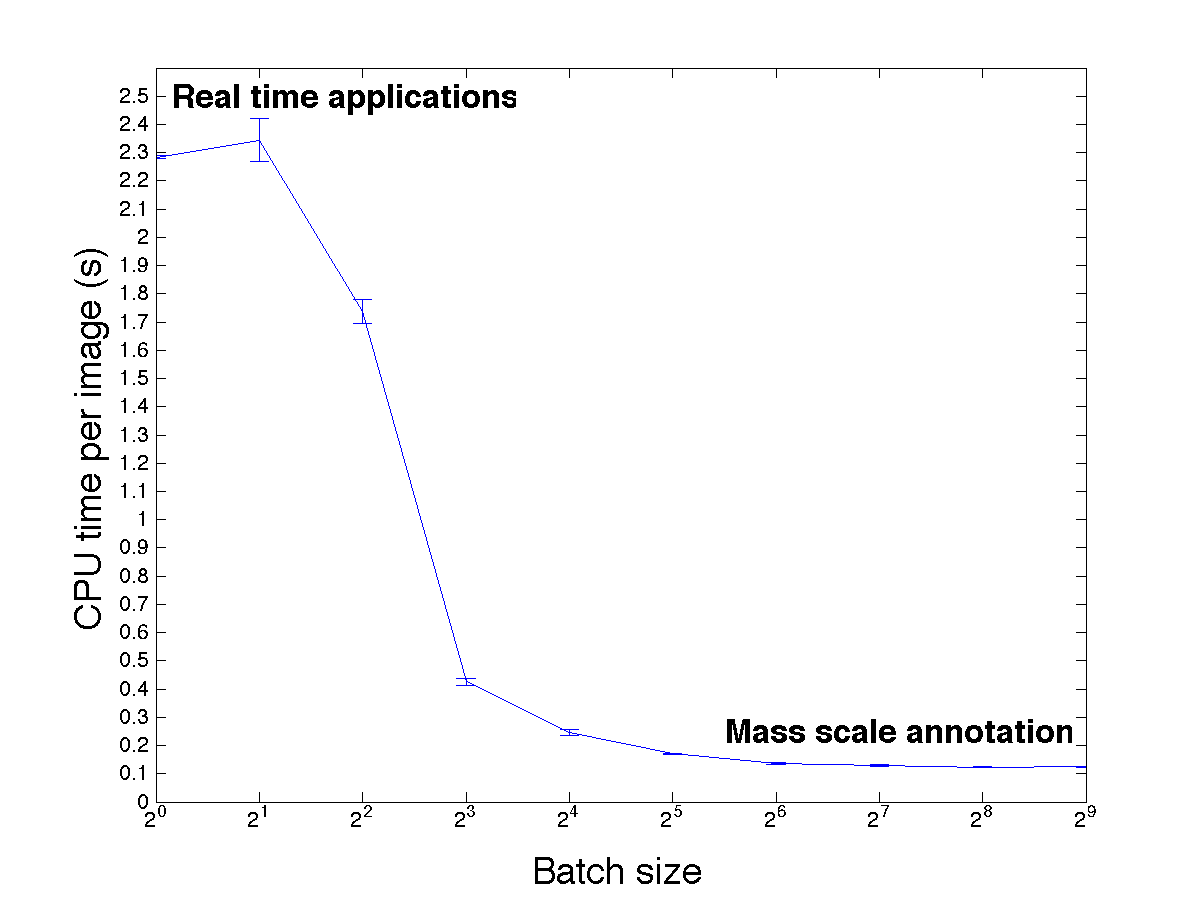
\includegraphics[width=0.48\textwidth]{img/eval_per_batch.png}
  \caption{CPU computational time per image for various batch sizes.}
\end{figure}
\begin{figure}[ht]
  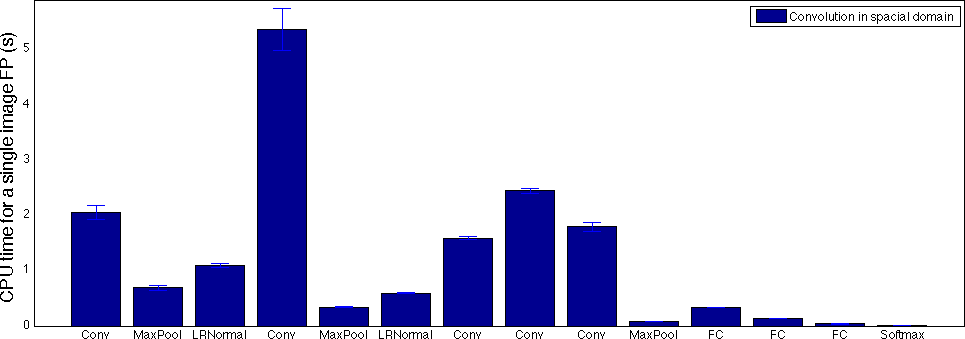
\includegraphics[width=0.48\textwidth]{img/eval_per_layer_per_batch_128_batch_size.png}
  \caption{Per layer breakdown of execution time for mini batch of size 128. Such size of mini batch gives optimal per image CPU time.}
\end{figure}
\begin{figure}[ht]
  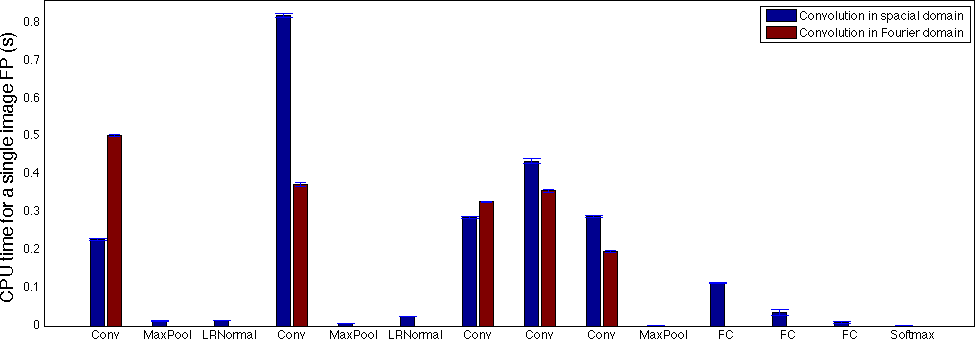
\includegraphics[width=0.48\textwidth]{img/eval_per_layer_per_batch_1_batch_size.png}
  \caption{Per layer breakdown of execution for mini batch of size 1. Use for real time applications.}
\end{figure}


\begin{figure}[ht]
  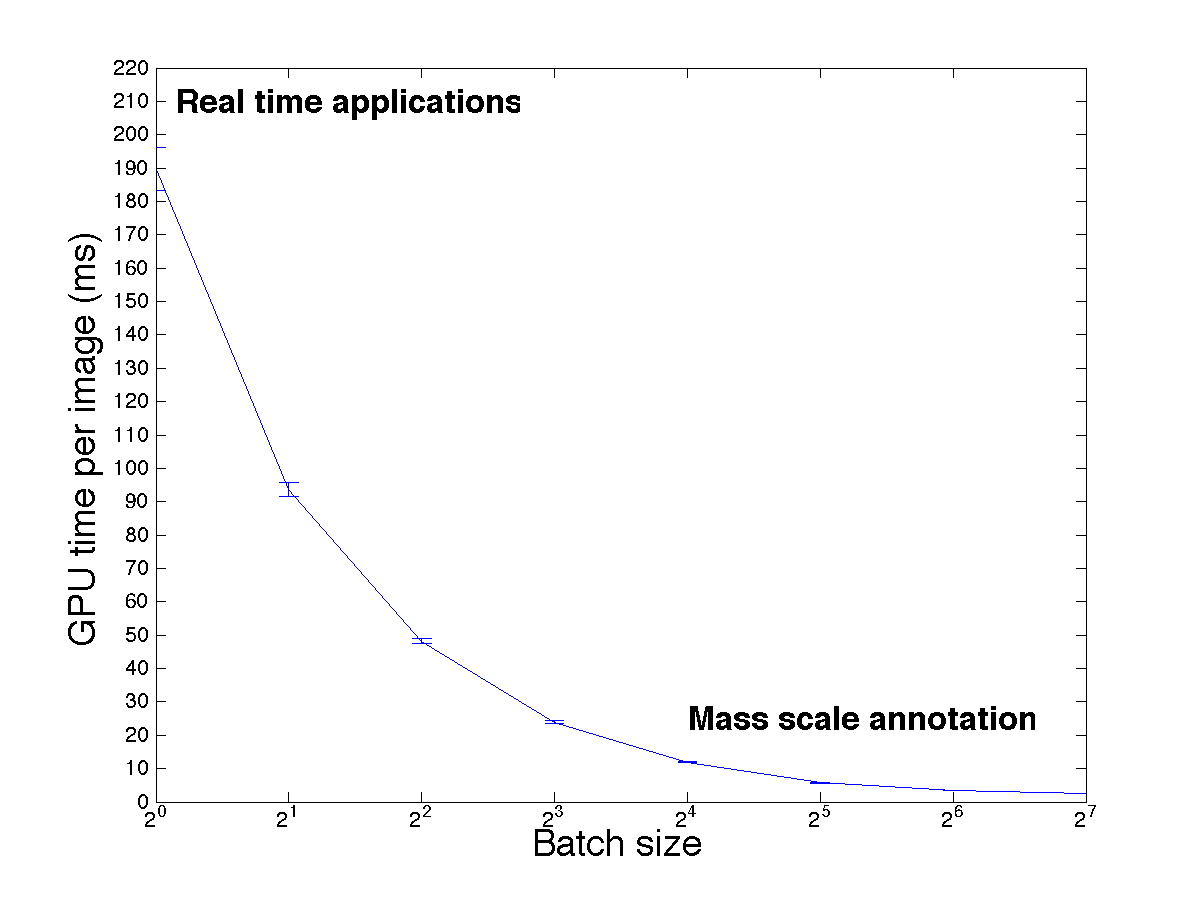
\includegraphics[width=0.48\textwidth]{img/eval_per_batch_GPU.png}
  \caption{GPU computational time per image for various batch sizes.}
\end{figure}
\begin{figure}[ht]
  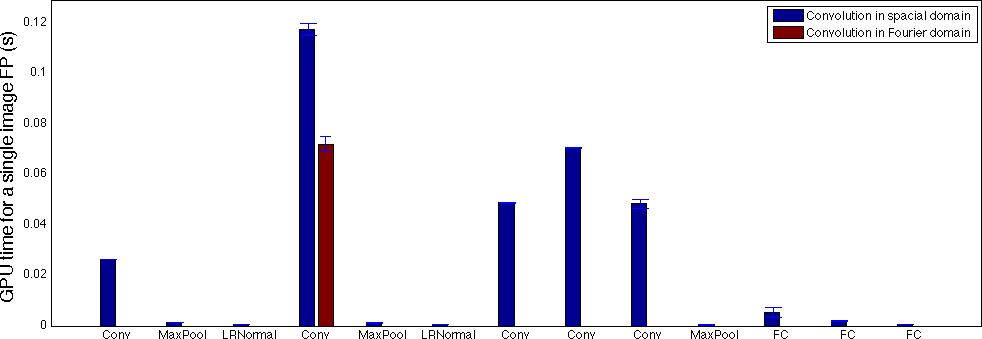
\includegraphics[width=0.48\textwidth]{img/eval_per_layer_per_batch_GPU_128_batch_size.png}
  \caption{Per layer breakdown of execution time for mini batch of size 128. Such size of mini batch gives optimal per image GPU time.}
\end{figure}

\subsection{Testing time}

on GPU: Michael can help.

on CPU

\subsubsection{Monochromatic}

\subsubsection{Linear combination of filters}

\subsubsection{Separable filters}


\subsection{ Denoising}
\begin{figure}[ht]
  \begin{minipage}[b]{0.48\linewidth}
  	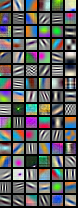
\includegraphics[width=\textwidth]{img/first.png}
  \end{minipage}
  \begin{minipage}[b]{0.48\linewidth}
  	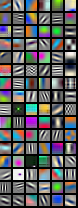
\includegraphics[width=\textwidth]{img/first_appr.png}
  \end{minipage}
  \caption{(Left) Original filters, (Right) approximated filters. (this pictures are too big, and should contain white separation).}
\end{figure}

\section{Implications} 

\subsection{Denoising Aspect}
we can improve training by simple linear denoting.

\subsection{Low-Rank training}
Low-rank to avoid over-fitting.


\section{Discussion}

\nocite{*}
\bibliography{bibliography}
\bibliographystyle{icml2014}


\end{document}






